

Als Datenbank wurde aus den in \autoref{datenbankauswahl} genannten Gründen MySQL ausgewählt.
Für die Erstellung der Datenbank entschieden sich die Autoren für die Verwendung eines Hilfswerkzeugs, in dem das Modell abgebildet und eine Befehlskette ausgegeben wird. Dadurch sollte eine Abweichung der Realisierung vom Modell vermieden und eine rasche prototypische Verifizierung ermöglicht werden. Aktuell existiert kein anerkannter Standard (wie z.B. UML) zur Beschreibung von Datenbanken, weshalb sich die Autoren für das Hilfswerkzeug Vertabelo entschieden. Dieses gibt die notwendigen SQL-Befehle aus, welche direkt für die Erstellung der Datenbank verwendet werden können. Weiterhin können die unter \url{vertabelo.com} angelegten Datenbankmodelle von mehreren Nutzern verwendet werden, was insbesondere für die geplante Weiterverwendung der Datenbank nützlich sein kann.
Die bereits in \autoref{img:db-schema} gezeigte Datenbank ist unter \cite{VertabeloDesignYourDatabase2018} abrufbar. Der daraus generierte SQL-Code wurde anschließend an die Anforderungen angepasst und befindet sich im Anhang  \autoref{a:datenbankerstellung}.


\subsection{Containerisierung}

Um das optionale Ziel der Containerisierung zu erreichen, wurde auf einen Standardcontainer der MySQL-Entwickler über Docker zurückgegriffen. Der Container zum Betrieb des Hubots basiert auf einem NodeJS Linux-Container, welcher mittels eines selbst entworfenen Dockerfiles erstellt wurde, welches in \autoref{lst:dockerfile} zu sehen ist.

% Die Autoren entschieden sich gegen den Bau eines eigenen Containers, um die Fehleranfälligkeit zu verringern und dokumentations- und supportkompatibel zu bleiben.

Docker ist eine Technologie zum Betrieb von Anwendungen in Containern, wobei jeder Container eine von den restlichen Containern isolierte Umgebung (Dateien, \linebreak Abhängigkeiten) erhält, dabei jedoch die Hardwareressourcen des Hostsystems mit anderen Containern teilt. Da diese Lösung wesentlich weniger Overhead bezüglich Speicher, Speicherplatz und Geschwindigkeit als eine Virtuelle Maschine bietet, eignen sich Container für die künstliche Abgrenzung vom Gesamtsystem und dadurch als einfach in den Produktiveinsatz zu überführende Lösung.

\subsubsection{Vergleich von Containerisierungslösungen}
Neben dem Einsatz der Containerlösung Docker wurden zu Projektbeginn Alternativen entsprechend \autoref{tab:docker-alternatives} betrachtet.

\begin{table}[H]
    \centering
    \begin{tabularx}{\textwidth}{|l|X|X|X|X|}
        \hline
        & \textbf{Docker} & \textbf{nativ} & \textbf{VirtualBox} & \textbf{Cloud} \\
        \hline
        Beschreibung & Umgebung für Linux-Container & lokale Installation der Anwendungen & Vollvirtuali- sierung inkl. Hardware & entfernte, dynamisch einsetzbare Ressourcen \\
        \hline
        Beispiel & docker pull mysql & apt install mysql & bitnami NodeJS VM & \url{heroku.com} \\
        \hline
        Geschwindigkeit     & $++$      & $+++$     & $+$   & $++++$ \\
        \hline
        Datensparsamkeit    & $++++$    & $++$      & $+++$ & $+$ \\
        \hline
        Portierbarkeit      & $++++$    & $+$       & $+++$ & $++$ \\
        \hline
        Persistenz          & $+$       & $+++$     & $++$  & $++++$ \\
        \hline
        \hline
        $\Sigma$            & 11        & 10        & 9     & 11 \\ 
        \hline
        \textbf{Ausschlusskriterium} & - & Testumgebung inhomogen, Serverinfrastruktur unbekannt & instabiles CLI (command line interface) & Datenschutz nicht gewährleistet, vendor-lock-in, laufende Kosten \\
        \hline
    \end{tabularx}
    \caption{Docker-Alternativen im Vergleich}
    \label{tab:docker-alternatives}
\end{table}

Der Vergleich der Docker-Alternativen erfolgte anhand einer positiven Gewichtung (Anzahl $+$) auf einer Skala von 1 bis 4. Dies ist für den groben Überblick ausreichend, bildet dabei aber keine detailliertere Gewichtung der Aspekte ab. Zur Abschätzung der Vor- und Nachteile reicht dieser grobe Vergleich jedoch aus. Die Gewichtung der Aspekte untereinander ist außerdem inhomogen. So ist die Anforderung der Datensparsamkeit z.B. wichtiger als die Geschwindigkeit. Daher sind die im folgenden näher erläuterten Punkte gesondert zu betrachten, da die Betrachtung der Summe über die Teilaspekte zum einen wenig aussagekräftig ist und zum anderen keine Form der Gewichtung der Vergleichskriterien beinhaltet.

\begin{itemize}
    \item Beispiel - ein charakteristischer Befehl/Referenz, siehe \cite{HubotDeploying2018}
    \item Geschwindigkeit - relative Zeit zur Ausführung der Anwendung
    \item Datensparsamkeit - Menge der ausgehenden Daten (weniger ist besser)
    \item Portierbarkeit - Grad der einfachen Portierung auf andere Systeme/Plattformen
    \item Persistenz - Möglichkeiten zur dauerhaften Datenspeicherung
\end{itemize}


\subsubsection{Entwicklungsumgebung mit Docker}

Basierend auf \autoref{img:deployment} ist die Systemumgebung für den Betrieb von Hubot mindestens aus den Komponenten Chatbot und Termindatenbank aufgebaut. Aus Gründen der Wartbarkeit, des fehlerminimierenden Betriebs und der offiziellen Empfehlung der Entwickler wird diese Trennung auch von den Docker-Containern aufrechterhalten.

Besondere Beachtung erfordert dabei die Verwaltung persistenter Daten, insbesondere der Datenbank. Da Docker-Container Daten standardmäßig nur flüchtig speichern, % Idempotenz kann man hier nicht wirklich sagen, da man die referenz auf einen container entfernen muss, bevor man ihn wieder starten kann, das ist gecheatet. finde ich dementsprechend gewagt
wird für den Erhalt der Datenbank ein persistentes Docker-Volume benötigt. Dafür wird ein Volume zwischen Hostsystem und Docker-Container eingebunden, sodass die Datenbank auch nach Beenden des Containers zur Verfügung steht.

Hinzu kommt ein weiterer Container zum Betrieb des eigentlichen Chatbots mittels NodeJS. Dieser wird mit dem gleichen virtuellen Netzwerk wie der DB-Container verbunden um Zugriff auf die Datenbank zu erhalten.

Weitere Einstellungen wie z.B. die zu öffnenden Ports folgen dem Paradigma \enquote{Convention over Configuration}. \cite{NicholasChenConventionConfiguration2006} Die Verbindung der Container untereinander erfolgt mittels docker-compose, in der docker-compose-Datei sind ebenfalls vordefinierte Standardwerte enthalten, welche schnell zum produktiven Einsatz führen (\cite{DockerInc.DockerCompose2018} und \autoref{lst:docker-compose}).
Dynamische Konfigurationen wie z.B. die UserID des Slackbots werden über entsprechende Umgebunsgvariablen in einer \verb+.env+-Datei übergeben und können problemlos während der Laufzeit geändert werden.

% docker-compose beschreiben


%hubot-docker bla


\subsection{Slackidentifizierung}

Die Identifizierung von Nutzern durch den Bot geschieht über die von Slack vergebene eindeutige Nutzeridentifizierungsnummer, welche über ein Nachrichtenobjekt innerhalb des Bots ausgelesen werden kann. Diese eindeutige Identifizierungsnummer wird durch den aufrufenden Nutzer in Slack in die Datenbank eingetragen, indem der Nutzer folgenden den Befehl aufruft: 
\texttt{@bob füge mich der Datenbank hinzu als <Vorname Nachname>}.

Der angegebene Name wird anschließend in der Nutzertabelle identifiziert und mit der SlackID verknüpft. Die Zuweisung kann nicht automatisch durch den in Slack angegebenen Namen geschehen, da dieser nicht gleich dem in der Datenbank als echten Namen eingetragenen Namen sein muss.


% anflanschung der slacknutzer-tabelle // vielleicht in eine separate db??? oder reicht ne tabelle / viele tabellen für viele plattformen aus

\subsection{Botrealisierung}
\subsubsection{Botname}
Da der Bot einen im deutschsprachigen Raum selten vorkommenden und zugleich kurzen und dadurch schnell zu schreibenden und leicht zu merkenden Namen erhalten sollte, entschieden sich die Autoren für den Namen Bob. Hierbei ist es nicht notwendig auf die Groß- und Kleinschreibung zu achten. Weiterhin wird der Bot im dynamischen Dropdownmenü innerhalb von Slack als Vorschlag angeboten, wenn dieser dem Raum hinzugefügt und direkt mittels einem \texttt{@}-Symbol adressiert wird. Die Autoren erhoffen sich dadurch eine einfachere Verwendung des Bots innerhalb der mobilen Applikation, da bei diesen die Schreibgeschwindigkeit geringer ist. Weiterhin kann dadurch eine größere Akzeptanz erreicht werden.

\subsubsection{Ereignisgesteuerte Aktionen}

Ereignisgesteuerte Aktionen werden nur ausgeführt, wenn ein Nutzer ein Ereignis auslöst. Der Bot interpretiert hierbei jede in den Chat geschriebene Nachricht und prüft diese auf ein Muster mithilfe eines regulären Ausdrucks. Da die Definitionen der ereignisgesteuerten Aktionen in der EBNF geschrieben wurden, können diese ohne umfangreiche Konvertierung mit einem regulären Ausdruck implementiert werden. Hierbei ist die Groß- und Kleinschreibung und die Anzahl an Leerzeichen zwischen den Schlagwörtern unwichtig.

\subsubsection{Zeitgesteuerte Aktionen}

Die zeitgesteuerten Aktionen beschränken sich auf die selbstständige Erinnerung an Termine durch den Bot. Der Bot darf in dieser Hinsicht keinen Zwischenspeicher besitzen, da neue Termine nicht durch den Bot eingetragen werden müssen und von einer externen Anwendung kommen können. Der gemeinsame Zugriffspunkt ist die Datenbank. Aus diesem Grund fragt der Bot die Datenbank periodisch ab.

Die Autoren legten eine zeitlich positive Abweichung von 5 Minuten als akzeptablen Wert bezüglich des echten Termins fest. Dieser entstand durch die Überlegung, wie groß die maximale Dauer für eine Abfrage an die Datenbank sein kann. Bei einer Teilnehmeranzahl von im $\o$ 10, einer Mitgliedsdauer von 50 Jahren und einer implementierungstechnisch pessimistisch angenommenen wöchentlichen Teilnahme an einer Veranstaltung pro Mitglied würden $52 \cdot 50 \cdot 10$ Terminschichteinträge vorhanden sein. Da eine Abfrage des nächsten Termins auf einem aktuellen Laptop $\approx 60\mu s$ dauert, ist eine obere Grenze von $52 \cdot 10 \cdot 50 \cdot 60 \mu s=1,56s=\varepsilon $ zu erwarten.

Der Bot fragt die Datenbank periodisch aller 3 Minuten auf nächstgelegene Termine ab, während die zu betrachtenden Termine in einer Zeitspanne von 5 Minuten liegen. Da der Bot eine maximale Abfragezeit von $\varepsilon + 3min$ hat, liegt der Abtastzeitpunkt selbst mit $\varepsilon$ immer innerhalb der 5 Minuten-Spanne. \autoref{querytiming} verdeutlicht dies.
 
\begin{figure}[htbp]
	\centering
	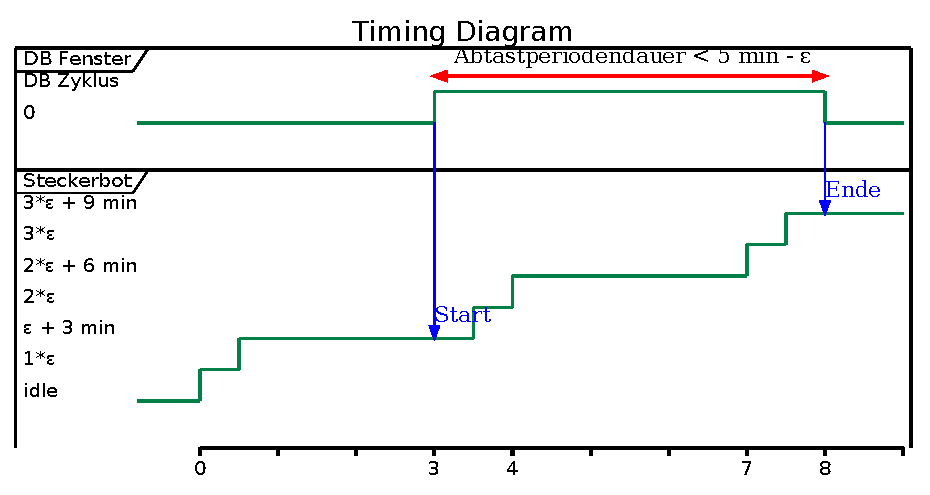
\includegraphics[width=1\textwidth,clip]{img/query.pdf}
	\caption{Zeitdiagramm für die Datenbankabfrage}
	\label{querytiming}
\end{figure}

Es ist zu erkennen, dass das Zeitfenster, in dem die Abfrage eines Termins stattfindet, an $t=3s$ beginnt und bei $t=8s$ endet, während der Bot mindestens einen Abtastzeitpunkt innerhalb der Zeitspanne besitzt. Die beiden Zeitpunkte liegen in der Grafik bei $t=2 \cdot \varepsilon + 2\cdot 3min$ und $t=3\cdot \varepsilon + 3\cdot 3min$.


%Anhang mit botcode dranheften

%wie erweiterbarkeit realisiert? - include module bla, file x
